\documentclass[11pt]{exam}
\usepackage{amsmath}
\usepackage{amsthm}
\usepackage{amssymb}
\newcommand{\myname}{Cael Howard} %Write your name in here
\newcommand{\myUCO}{cthoward} 
\newcommand{\myhwtype}{Homework}
\newcommand{\myhwnum}{1} %Homework set number
\newcommand{\myclass}{Compsci 166}
\newcommand{\mylecture}{}
\newcommand{\mysection}{}

% Prefix for numedquestion's
\newcommand{\questiontype}{Question}


% Use this if your "written" questions are all under one section
% For example, if the homework handout has Section 5: Written Questions
% and all questions are 5.1, 5.2, 5.3, etc. set this to 5
% Use for 0 no prefix. Redefine as needed per-question.
\newcommand{\writtensection}{0}

\usepackage{amsmath, amsfonts, amsthm, amssymb}  % Some math symbols
\usepackage{enumerate}
\usepackage{enumitem}
\usepackage{graphicx}
\usepackage{hyperref}
\usepackage[all]{xy}
\usepackage{wrapfig}
\usepackage{fancyvrb}
\usepackage[T1]{fontenc}
\usepackage{listings}
\usepackage{accents}
\usepackage{braket}
\usepackage{tikz}
\usepackage{commath}

\usepackage{centernot}
\usepackage{mathtools}
\DeclarePairedDelimiter{\ceil}{\lceil}{\rceil}
\DeclarePairedDelimiter{\floor}{\lfloor}{\rfloor}
\DeclarePairedDelimiter{\card}{\vert}{\vert}


\setlength{\parindent}{0pt}
\setlength{\parskip}{5pt plus 1pt}
\pagestyle{empty}

\def\indented#1{\list{}{}\item[]}
\let\indented=\endlist

\newcounter{questionCounter}
\newcounter{partCounter}[questionCounter]

\newenvironment{namedquestion}[1][\arabic{questionCounter}]{%
    \addtocounter{questionCounter}{1}%
    \setcounter{partCounter}{0}%
    \vspace{.2in}%
        \noindent{\bf #1}%
    \vspace{0.3em} \hrule \vspace{.1in}%
}{}

\newenvironment{numedquestion}[0]{%
	\stepcounter{questionCounter}%
    \vspace{.2in}%
        \ifx\writtensection\undefined
        \noindent{\bf \questiontype \; \arabic{questionCounter}. }%
        \else
          \if\writtensection0
          \noindent{\bf \questiontype \; \arabic{questionCounter}. }%
          \else
          \noindent{\bf \questiontype \; \writtensection.\arabic{questionCounter} }%
        \fi
    \vspace{0.3em} \hrule \vspace{.1in}%
}{}

\newenvironment{alphaparts}[0]{%
  \begin{enumerate}[label=\textbf{(\alph*)}]
}{\end{enumerate}}

\newenvironment{arabicparts}[0]{%
  \begin{enumerate}[label=\textbf{\arabic{questionCounter}.\arabic*})]
}{\end{enumerate}}

\newenvironment{questionpart}[0]{%
  \item
}{}

\newcommand{\bravec}[2]{\begin{bmatrix} #1 & #2 \end{bmatrix}}

\newcommand{\ketvec}[2]{\begin{bmatrix} #1 \\ #2 \end{bmatrix}}

\newcommand{\answerbox}[1]{
\begin{framed}
\vspace{#1}
\end{framed}}

\pagestyle{head}

\headrule
\header{\textbf{\myclass\ \mylecture\mysection}}%
{\textbf{\myname\ (\myUCO)}}%
{\textbf{\myhwtype\ \myhwnum}}

\begin{document}
\thispagestyle{plain}
\begin{center}
  {\Large \myclass{} \myhwtype{} \myhwnum} \\
  \myname{} (\myUCO{}) \\
  \today
\end{center}


%Here you can enter answers to homework questions

\begin{numedquestion}
    \textbf{Problem Statement:}\\
    Frankie the frog lives in a pond with two lily pads, east and west. One day, she found two coins at the bottom of the pond and has placed one on each of the two lily pads. Every morning, Frankie flips the coin on the lily pad she spent her last day on, and jumps to the other lily pad if it lands heads. If the coin is tails, she stays on her lily pad for the day.

    The state space is E and W, corresponding to the lily pad Frankie spends her day on. We cannot assume that the coins are fair, as we do not know where they came from! They could be weighted in very different ways. Let’s call the probability that the east coin lands on heads to be $p$ and the probability that the west coin lands on heads to be $q$.
    \vspace{2em}

    \textbf{1.1)} On day one, Frankie is on the east lily pad. How can we express this fact using a probability vector?

    \vspace{1em}
    \textbf{Answer:}\\
    We will define east state space E and W as follows:
    \begin{align*}
        | E \rangle &= \begin{bmatrix}
                        1 \\
                        0
                        \end{bmatrix} \\
        | W \rangle &= \begin{bmatrix}
            0 \\
            1
            \end{bmatrix}
    \end{align*}
    Therefore, the probability vector representing the fact that Frankie is on the east lily pad is $\begin{bmatrix} 1 \\ 0 \end{bmatrix} \\$
    \vspace{2em}

    \textbf{1.2) } Write down the stochastic matrix that corresponds to Frankie's game.
    \vspace{1em}

    \textbf{Answer:}\\
    The stochastic matrix that corresponds to this game is as follows:
    \begin{center}
    $\begin{bmatrix}
    1-p & q \\
    p & 1-q
    \end{bmatrix}$
    \end{center}
    \newpage
    \textbf{1.3)} Gently place Frankie on the east lily pad and leave the pond for 1 day. Write down the probability vector that represents our best guess for Frankie's location. 
    \vspace{1em}

    \textbf{Answer:}\\
    The probability vector is:
    \begin{center}
      $\begin{bmatrix}
        1-p\\
        p
      \end{bmatrix}$
    \end{center}
    \vspace{1em}

    \textbf{1.4)} What if instead of 1 day, we left Frankie on the east lily pad and left for 2 days. What is the probability vector that represents our best guess for Frankie's location?
    \vspace{1em}

    \textbf{Answer:}
    \begin{align*}
      \begin{bmatrix}
        1-p & q\\
        p & 1-q
      \end{bmatrix}^{2}
      \begin{bmatrix}
      1-p\\
      p
      \end{bmatrix}
      =
      \begin{bmatrix}
        p^2 - 2 p + qp + 1 \\
        2p -p^2 -pq
      \end{bmatrix}
    \end{align*}
    \vspace{1em}

    \textbf{1.5)} We find another frog Arnold with his own pair of lily pads too, which we will call the north and south lily pads. They also each have coins, each with probability r and s of being heads. What is the probability vector that represents the fact that Arnold is on the north lily pad?
    \vspace{1em}

    \textbf{Answer:}\\
    We will define the north lily pad state as
    \begin{center}
    $\ket{N}=
    \begin{bmatrix}
    1\\
    0
    \end{bmatrix}
    $
    \end{center}
    Therefore, the probability vector representing Arnold being on the north lily pad is $\begin{bmatrix}
    1\\0
    \end{bmatrix}
    $
    \vspace{1em}

    \textbf{1.6)} We could independently track Frankie and Arnold's locations, but we can also combine the state spaces to describe both of their states at once. What is the probability vector that describes Frankie on the west lily pad and Arnold on the north lily pad?
    \vspace{1em}
    
    \textbf{Answer:}
    \begin{align*}
      \begin{bmatrix}
        0\\1
      \end{bmatrix}
      \otimes 
      \begin{bmatrix}
        1\\0
      \end{bmatrix}
      =
      \begin{bmatrix}
        0\\0\\1\\0
      \end{bmatrix}
    \end{align*}
    \newpage
    \textbf{1.7)} Suppose we place Frankie onthe west lily pad and Arnold on the north lily pad, and leave the pond for a day. What is the probability vector that represents our best guess for the state of the frogs after one day?

    \textbf{Answer:}
    \begin{align*}
      \begin{bmatrix}
        q\\1-q
      \end{bmatrix}
      \otimes
      \begin{bmatrix}
        1-r\\r
      \end{bmatrix}
      =
      \begin{bmatrix}
        q-qr\\qr\\1-q-r+qr\\r-qr
      \end{bmatrix}
    \end{align*}
    \vspace{1em}

    \textbf{1.8)}\\
    \vspace{-4em}
    \begin{figure}[ht]
    \centering
    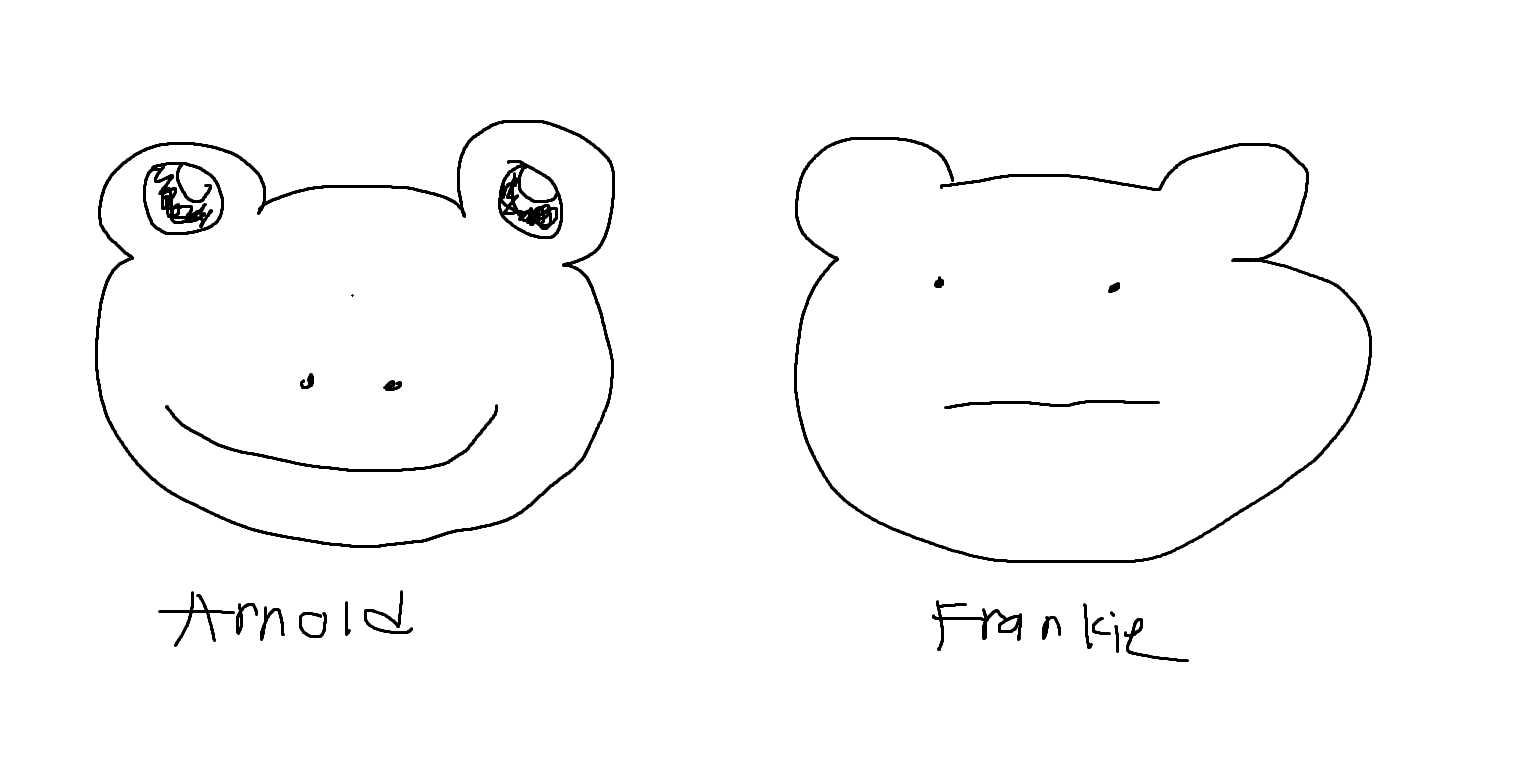
\includegraphics[width=0.5\textwidth]{src/hw1q8.png}
    \end{figure}
\end{numedquestion}

\begin{numedquestion}
  \textbf{2.1)} Write down the two solutions to $z^2 = 1$ in the standard notation of complex numbers.
  \vspace{1em}

  \textbf{Answer:}
  \begin{align*}
    z^2 &= 1\\
    z &= \sqrt{1}\\
    z &= \pm 1
  \end{align*}
  
  \newpage
  \textbf{2.2)} What are the $\theta$ if we write the above two solutions in polar notation, that is in the form $\text{cos} \theta + i\text{sin}\theta = e^{i\theta}$. Draw the solutions in the complex plane and label the angle $\theta$ they form with the positive real axis. Verify that for each of the $\theta$, you get $(e^{i\theta})^2 = 1$.
  \vspace{1em}

  \textbf{Answer:}\\
  The two answers are $z=\text{cos}0 + i\text{sin}(0) = e^{0i}, \text{cos}(\pi) + i\text{sin}(\pi i) = e^{\pi i}$.\\
  \begin{figure}[ht]
    \centering
    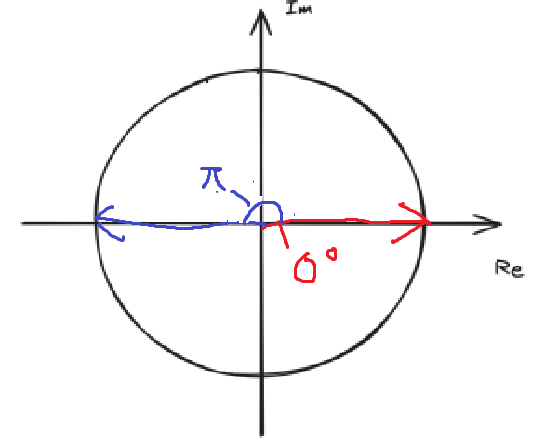
\includegraphics[width=0.4\textwidth]{src/hw1q13.png}
  \end{figure}

  \textbf{Verify}:
  $$e^{2 * 0i} = e^0 = 1$$
  $$e^{2\pi i} = \text{cos}(2\pi) + i \text{sin}(2\pi) = 1 + 0 = 1$$
  \vspace{1em}

  \textbf{1.3)} What are the three solutions to $z^3 = 1$?
  \vspace{1em}

  \textbf{Answer:}\\
  \begin{minipage}[t]{0.45\textwidth} 
    \vspace{0pt} % Ensure proper alignment at the top
    \begin{align*}
      z^3 &= 1\\
      e^{3i\theta} &= 1\\
      \cos(3\theta) + i\sin(3\theta) &= 1\\
      3\theta &= 2\pi k\\
      \theta &= \frac{2\pi}{3}k\\
      \theta &= 0, \frac{2\pi}{3}, \frac{4\pi}{3}\\
      z &= e^{0}, e^{i\frac{2\pi}{3}}, e^{i\frac{4\pi}{3}}
    \end{align*}
\end{minipage}
\hfill
\begin{minipage}[t]{0.5\textwidth}
    \vspace{0pt} % Ensure proper alignment at the top
    \centering
    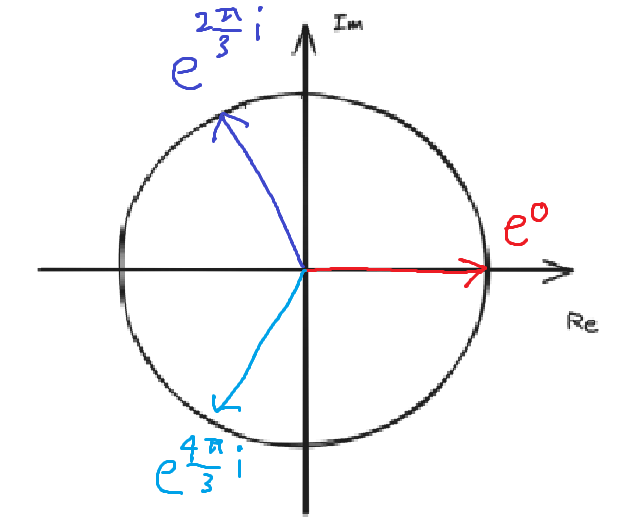
\includegraphics[width=0.9\textwidth]{src/hw1q14.png}
\end{minipage}
\newpage
\textbf{1.4)} Let the three solutions from the previous problem be $1, \omega_3,\omega_{3}$ going in counter clockwise order. Verify that the second solution does indeed square to be the third solution.
\vspace{1em}

\textbf{Answer:}
\begin{align*}
(e^{i\frac{2\pi}{3}})^2 &= e^{i\frac{4\pi}{3}}\\
e^{i\frac{4\pi}{3}} &= e^{i\frac{4\pi}{3}}
\end{align*}

\textbf{1.5)} We call solutions to the equation $z^{n} = 1$ the $n$-th roots of unity. Of particular interest is the first one in the counter clockwise direction after $1$, which we call $\omega_n$. All the other $n$-th roots of unity can be constructed once this is known. What is a general form for the value of $w_n$? As a hint, you will want to use polar coordinates.
\vspace{1em}

\textbf{Answer:}\\
General form for the solutions for the $n$-th roots of unity is $e^{i\frac{2\pi}{n}k}$ where $k$ is an integer.
\vspace{1em}

\textbf{1.6)} What do you get when you add all three 3rd roots of unity? Briefly justify your solution by drawing the addition.
\vspace{1em}

\textbf{Answer:}\\
If you add all 3rd roots of unity, the resulting vector is $\vec{0}$.
\begin{figure}[ht]
  \centering
  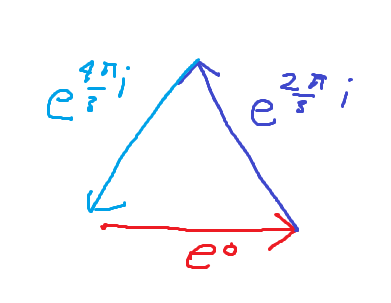
\includegraphics[width=0.4\textwidth]{src/hw1q16.png}
\end{figure}
\vspace{1em}

\textbf{1.7)} Do you get the same result as above if adding up all the 4-th roots of unity? What if we add all the $n$-th roots of unity?
\vspace{1em}

\textbf{Answer:}\\
For all $n$, the sum of the $n$-th roots of unity is $\vec{0}$.

\end{numedquestion}
\newpage

\begin{numedquestion}
    Consider the following quantum state:
    \vspace{1em}

    $\ket{\psi} = \frac{i}{\sqrt{2}}\ket{0} - \frac{1}{\sqrt{2}}\ket{1}$
    \vspace{1em}

    \textbf{3.1)} Verify that $\ket{\psi}$ is indeed a quantum state.
    \begin{align*}
    \norm{\ket{\psi}} &= \sqrt{\abs{\frac{i}{\sqrt{2}}}^2 + \abs{\frac{-1}{\sqrt{2}}}^2}\\
    &= \sqrt{1/2 + 1/2}\\
    &= 1
    \end{align*}
    Since $\ket{\psi}$ is a unit vector with comlex amplitudes, it is a quibit.
    \vspace{1em}

    \textbf{3.2)} If we measure $\ket{\psi}$, what is the probability we measure $\ket{0}$?

    \textbf{Answer:}\\
    The probability we measure $\ket{0}$ is $\alpha_0^2$ or:
    \begin{align*}
    \alpha^2 &= \abs{\frac{i}{\sqrt{2}}}^2\\
    &= \frac{1}{2}
    \end{align*}
    \vspace{1em}

    \textbf{3.3)} Suppose we did observe $\ket{0}$, what is the state of the quibit after the measurement?

    \textbf{Answer:}\\
    The quibit collapses to $\ket{0}$.
    \vspace{1em}

    \textbf{3.4)} Find a state that is orthogonal to $\ket{\psi}$

    \textbf{Answer:}\\
    We will find a $\ket{\phi}$ such that $\braket{\phi | \psi} = 0$:
    \begin{align*}
    \braket{\phi | \psi} &= 0\\
    \alpha_0^{*}\frac{i}{\sqrt{2}} + \alpha_{1}^{*}\frac{-i}{\sqrt{2}} &= 0\\
    \alpha_0^{*}\frac{i}{\sqrt{2}} &= \alpha_{1}^{*}\frac{i}{\sqrt{2}}\\
    \alpha_0^*, \alpha_1^* &= \frac{i}{\sqrt{2}},\frac{i}{\sqrt{2}}
    \end{align*}
    Therefore, the vector that is orthogonal to $\ket{\psi}$ is $\ket{\phi} = \begin{bmatrix}
        -i/\sqrt{2}\\
        -i/\sqrt{2}
    \end{bmatrix}$
    \vspace{1em}
    \newpage
    Consider the following quantum state

    $\ket{\psi} = (\frac{\sqrt{3}}{4} + i\frac{1}{4})\ket{0} + (-\frac{\sqrt{3}}{4} + i\frac{3}{4})\ket{1}$
    \vspace{1em}
    
    \textbf{3.5)} Verify that $\ket{\psi}$ is a quantum state:
    \begin{align*}
    \norm{\ket{\psi}} &= \sqrt{(\frac{\sqrt{3}}{4} + i\frac{1}{4})(\frac{\sqrt{3}}{4} - i\frac{1}{4}) + (-\frac{\sqrt{3}}{4} + i\frac{3}{4})((-\frac{\sqrt{3}}{4} - i\frac{3}{4}))}\\
    &= \sqrt{(\frac{3}{16} + \frac{1}{16}) + (\frac{3}{16} + \frac{9}{16})}\\
    &= 1
    \end{align*}
    Since the norm of $\ket{\psi}$ is $1$ and it can be represented as a vector with two complex amplitudes, it is a quantum state.
    \vspace{1em}

    \textbf{3.6)} What is the probability that we measure $\ket{0}$ if we measure in the standard basis? What is the state after the measurement?
    
    \textbf{Answer:}\\
    The probability that we measure $\ket{\psi}$ is $\abs{\frac{\sqrt{3}}{4} + i\frac{1}{4}}^2$ which is $\frac{1}{4}$. The quibit collapses to $\ket{0}$.
    \vspace{1em}

    \textbf{3.7)} Find a state orthogonal to $\ket{\psi}$.

    We will find $\ket{\phi} = \begin{bmatrix} \alpha_0 \\ \alpha{1}\end{bmatrix}$ such that $\braket{\phi^* | \psi} = 0$.
    \begin{align*}
    \bravec{\alpha_0^*}{\alpha_1^*}\ketvec{\frac{\sqrt{3}}{4}+i\frac{1}{4}}{-\frac{\sqrt{3}}{4} + i\frac{3}{4}} &= 0\\
    \alpha_0^*,\alpha_1^* &= \frac{\sqrt{3}}{4} - i\frac{3}{4}, \frac{\sqrt{3}}{4}+i\frac{1}{4}
    \end{align*}
    Therefore we get that:
    $$\ket{\phi} = \ketvec{\frac{\sqrt{3}}{4} + i\frac{3}{4}}{\frac{\sqrt{3}}{4}-i\frac{1}{4}}$$
    \vspace{1em}

    \textbf{3.8)} Consider the state $e^{i\pi/4}\ket{\psi}$. That is, multiply the amplitudes by $e^{i\pi/4}\ket{\psi}$. What is the probability that we measure $\ket{0}$ if we measure in the standard basis?
    \vspace{1em}

    First we find the value of $e^{i\pi/4} = \frac{1}{\sqrt{2}} + i\frac{1}{\sqrt{2}}$. Now, we will rewrite $\alpha_0$ as 
    \begin{align*}
      \frac{\sqrt{3}}{4}+i\frac{1}{4} &= \frac{1}{2}(\frac{\sqrt{3}}{2} + i\frac{1}{2})\\
      &= \frac{1}{2}e^{i\pi/6}
    \end{align*}
    Now, to find the probability of measuring $\ket{0}$, we take the square of the norm of the amplitude:
    \begin{align*}
    \abs{e^{i\pi/6}\alpha_0}^2 &= \abs{e^{i\pi/4}\frac{1}{2}e^{i\pi/6}}^2\\
    &= \abs{\frac{1}{2}e^{i5\pi/12}}^2\\
    &= \frac{1}{4} (\text{cos}(5\pi/12) + i\text{sin}(5\pi/12))(\text{cos}(5\pi/12) - i\text{sin}(5\pi/12))\\
    &= \frac{1}{4}(\text{cos}^2(5\pi/12) + \text{sin}^2(5\pi/12))\\
    &= \frac{1}{4}
    \end{align*}
\end{numedquestion}
\vspace{1em}

\begin{numedquestion}
  \textbf{4.2)} Define the two quibit states $\ket{\phi}$ and $\ket{psi}$ as:

  $\ket{\psi} = \frac{\ket{0} + 3i\ket{1}}{\sqrt{10}}$ and $\ket{\phi} = \frac{2\ket{0} - i\ket{1}}{\sqrt{5}}$
  \vspace{1em}

  What is $\braket{\phi | \psi}$?

  \textbf{Answer}:
  \begin{align*}
    \braket{\phi | \psi} &= \frac{2}{\sqrt{50}} + \frac{3i^2}{\sqrt{50}}\\
    &= -\frac{1}{\sqrt{50}}
  \end{align*}

  What is $\braket{\psi | \phi}$?

  \textbf{Answer:}
  \begin{align*}
    \braket{\phi | \psi} &= \frac{2}{\sqrt{50}} + \frac{3i^2}{\sqrt{50}}\\
    &= -\frac{1}{\sqrt{50}}
  \end{align*}
  \vspace{1em}

  \textbf{4.3)} A quibit state should be normalized, meaning the norm should be 1: $\norm{\ket{\phi}} = 1$. The following state $\ket{\phi}$ is $\textbf{not}$ normalized. Find a constant $N$ such that $\frac{1}{N}\ket{\phi}$ is normalized.

  $\ket{\phi} = 3\ket{0} - i\ket{1}$
  
  \textbf{Answer:}\\
  To find the normalized vector, we divide the non-normalized vector by  its norm. The norm for $\ket{\phi}$ is $\sqrt{\braket{\phi | \phi}} = \sqrt{\bravec{3}{i} \ketvec{3}{-i}} = \sqrt{10}$. Therefore, the normalized vector would be $\ket{\psi} = \frac{1}{\sqrt{10}}\ket{\phi}$.
  \vspace{1em}

  \textbf{4.4)} Define
  $\ket{i} = \frac{\ket{0}+i\ket{1}}{\sqrt{2}}$ and $\ket{-i} = \frac{\ket{0}-i\ket{1}}{\sqrt{2}}$. Prove that the pair of state $\ket{i}, \ket{-i}$ for an orthonormal basis.

  $\ket{i} = \ketvec{1/\sqrt{2}}{i/\sqrt{2}}$ $\ket{-i} = \ketvec{1/\sqrt{2}}{-i/\sqrt{2}}$

  \textbf{Answer:}\\
  First we will show that the norm of both states is $1$.

  $\sqrt{\braket{i|i}} = \frac{1}{2} - \frac{i^2}{2} = 1$\\
  $\sqrt{\braket{-i|-i}} = \frac{1}{2} - \frac{i^2}{2} = 1$

  Now, we demonstrate that the two vectors are orthogonal.
  $$\braket{i | -i} = 1/2 + i^2/2 = 0$$
  Thus, the pair of states form an orthonormal bases.
\end{numedquestion}



\end{document}
